\section{Measurement Method}

The experimental setup consists of a signal source, two piezoelectric
transducers $S_1$ and $S_2$, and oscilloscope arranged as shown in Figure~
\ref{app}.

\begin{figure}[H]
    \centering
    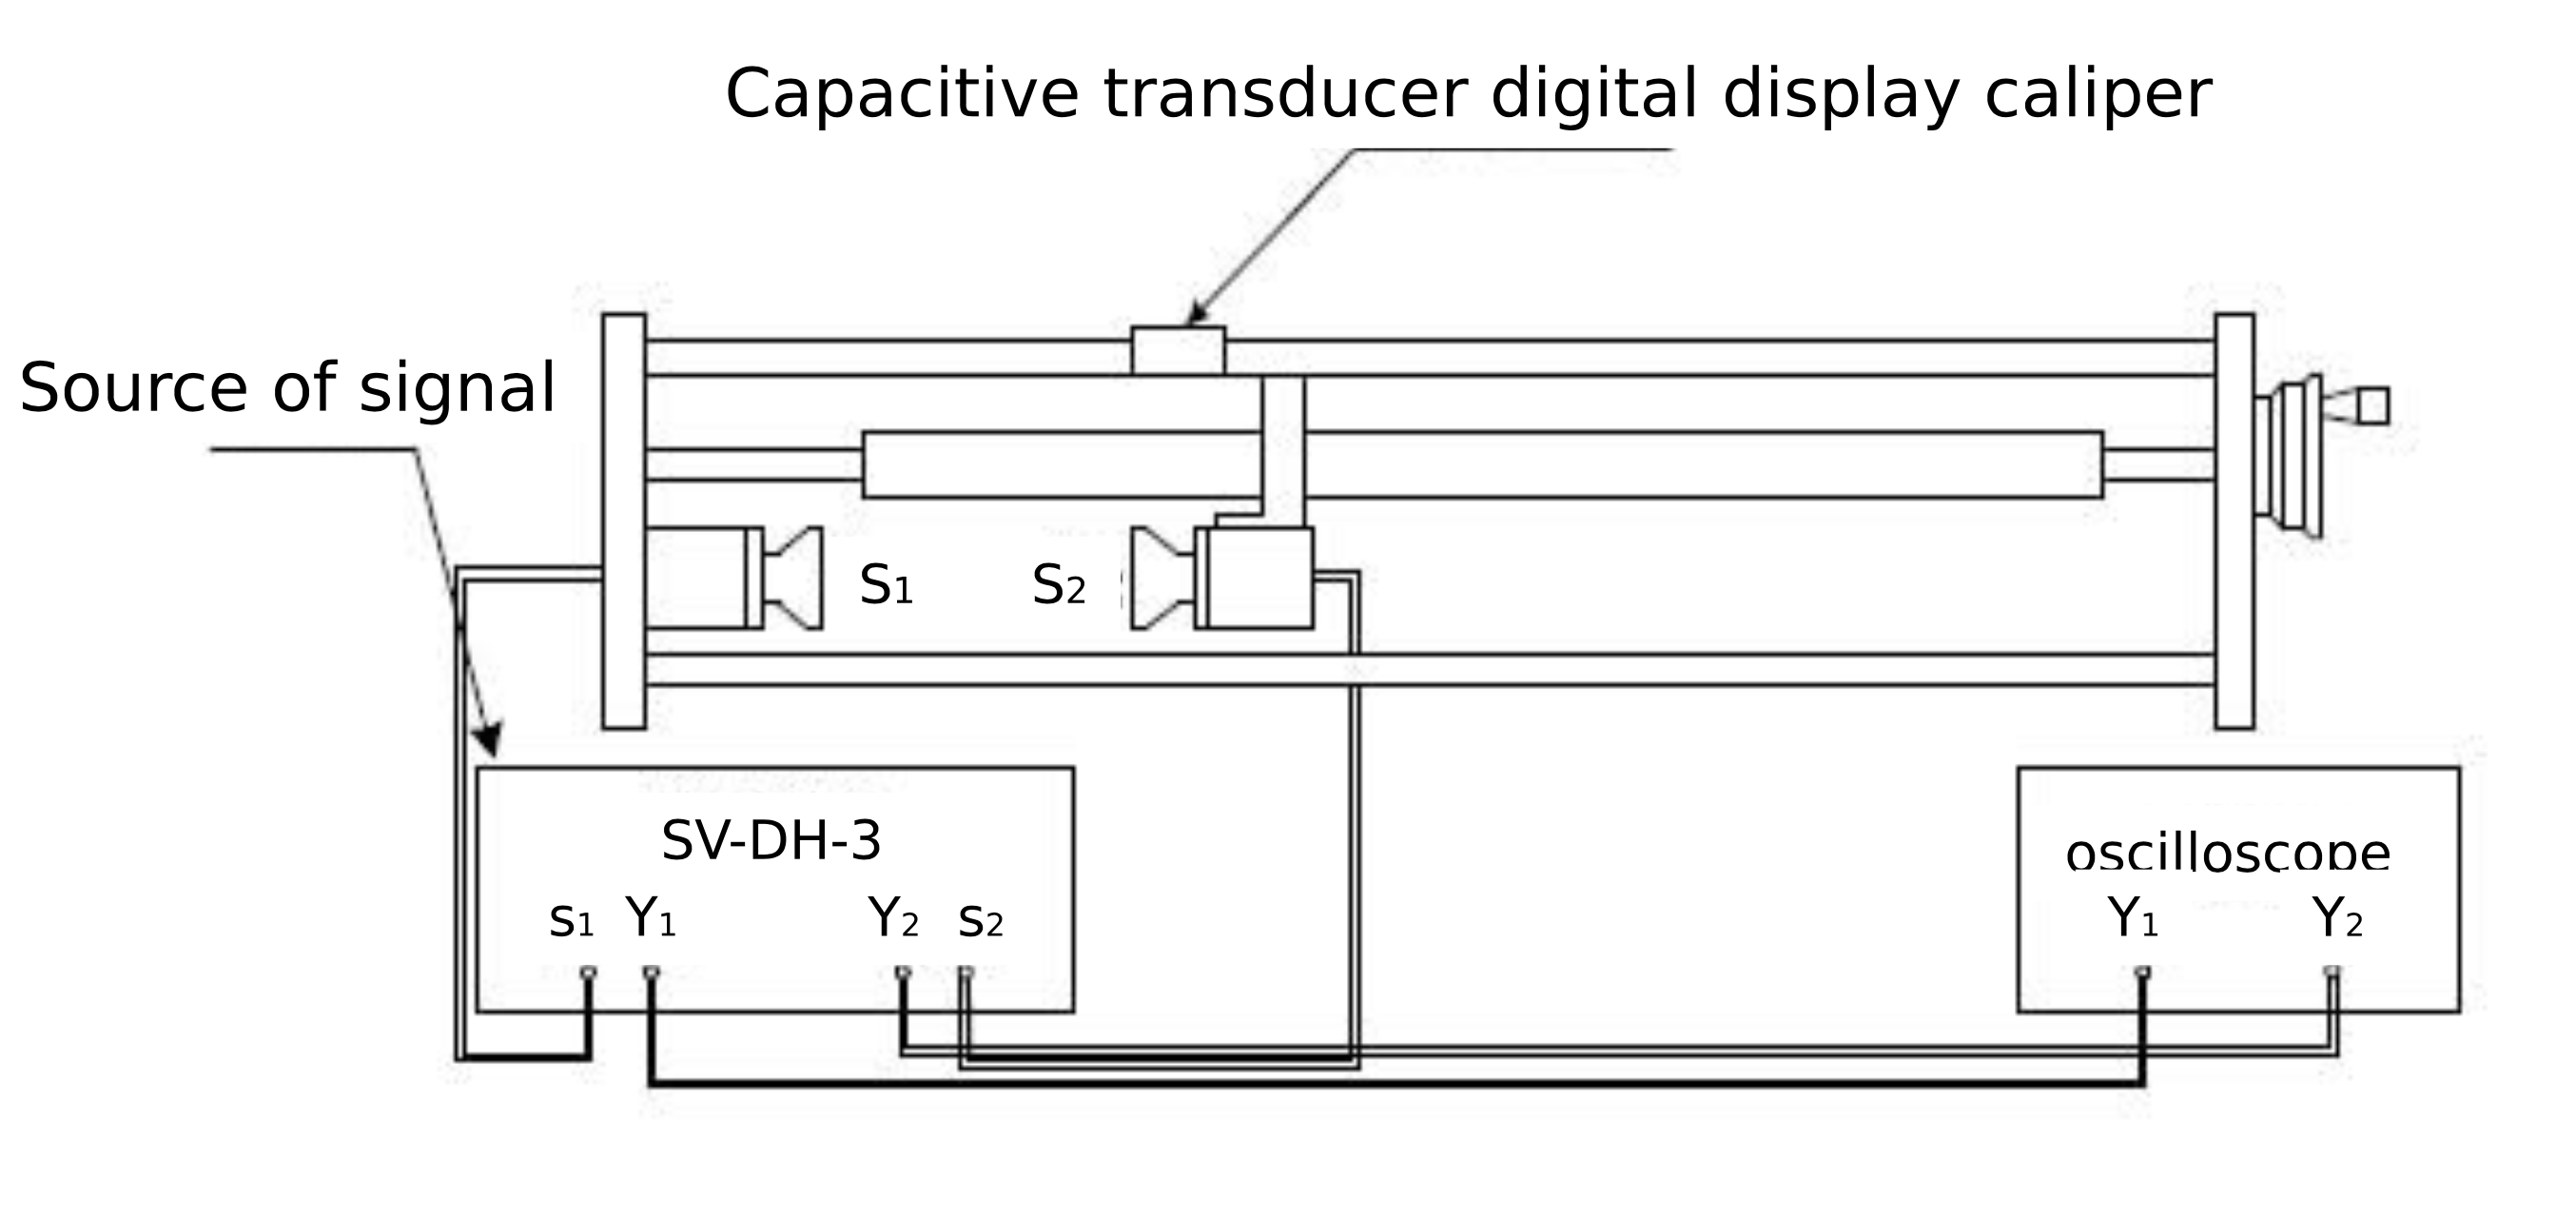
\includegraphics[width=12cm]{fig/es1}
    \caption{Experimental setup}\label{app}
\end{figure}


\subsubsection{Resonance method}

The elements $S_1$ and $S_2$ are the wave source and the receiver (also
reflector), respectively, placed a distance $L$ from each other. If they are
arranged parallel to each other, the sound wave is reflected. If 

\begin{equation}
    L=n\frac{\lambda}{2},
    \label{equ_res}
\end{equation}

where $n=1,2,\cdots,$ \emph{i.e.} the distance is a multiple of
half-wavelength, standing waves will form, and maximum output power will be
observed in the oscillograph (Figure 2). The distance between two successive
maxima ($L_{i+1} - L_i$) is always $\lambda/2$. After the position
corresponding to each maximum is measured, it is easy to find the wavelength
and then the speed of sound by using Eq.~\ref{vlf}. The frequency $f$ is
displayed directly on the signal generator. 

\begin{figure}[H]
    \centering
    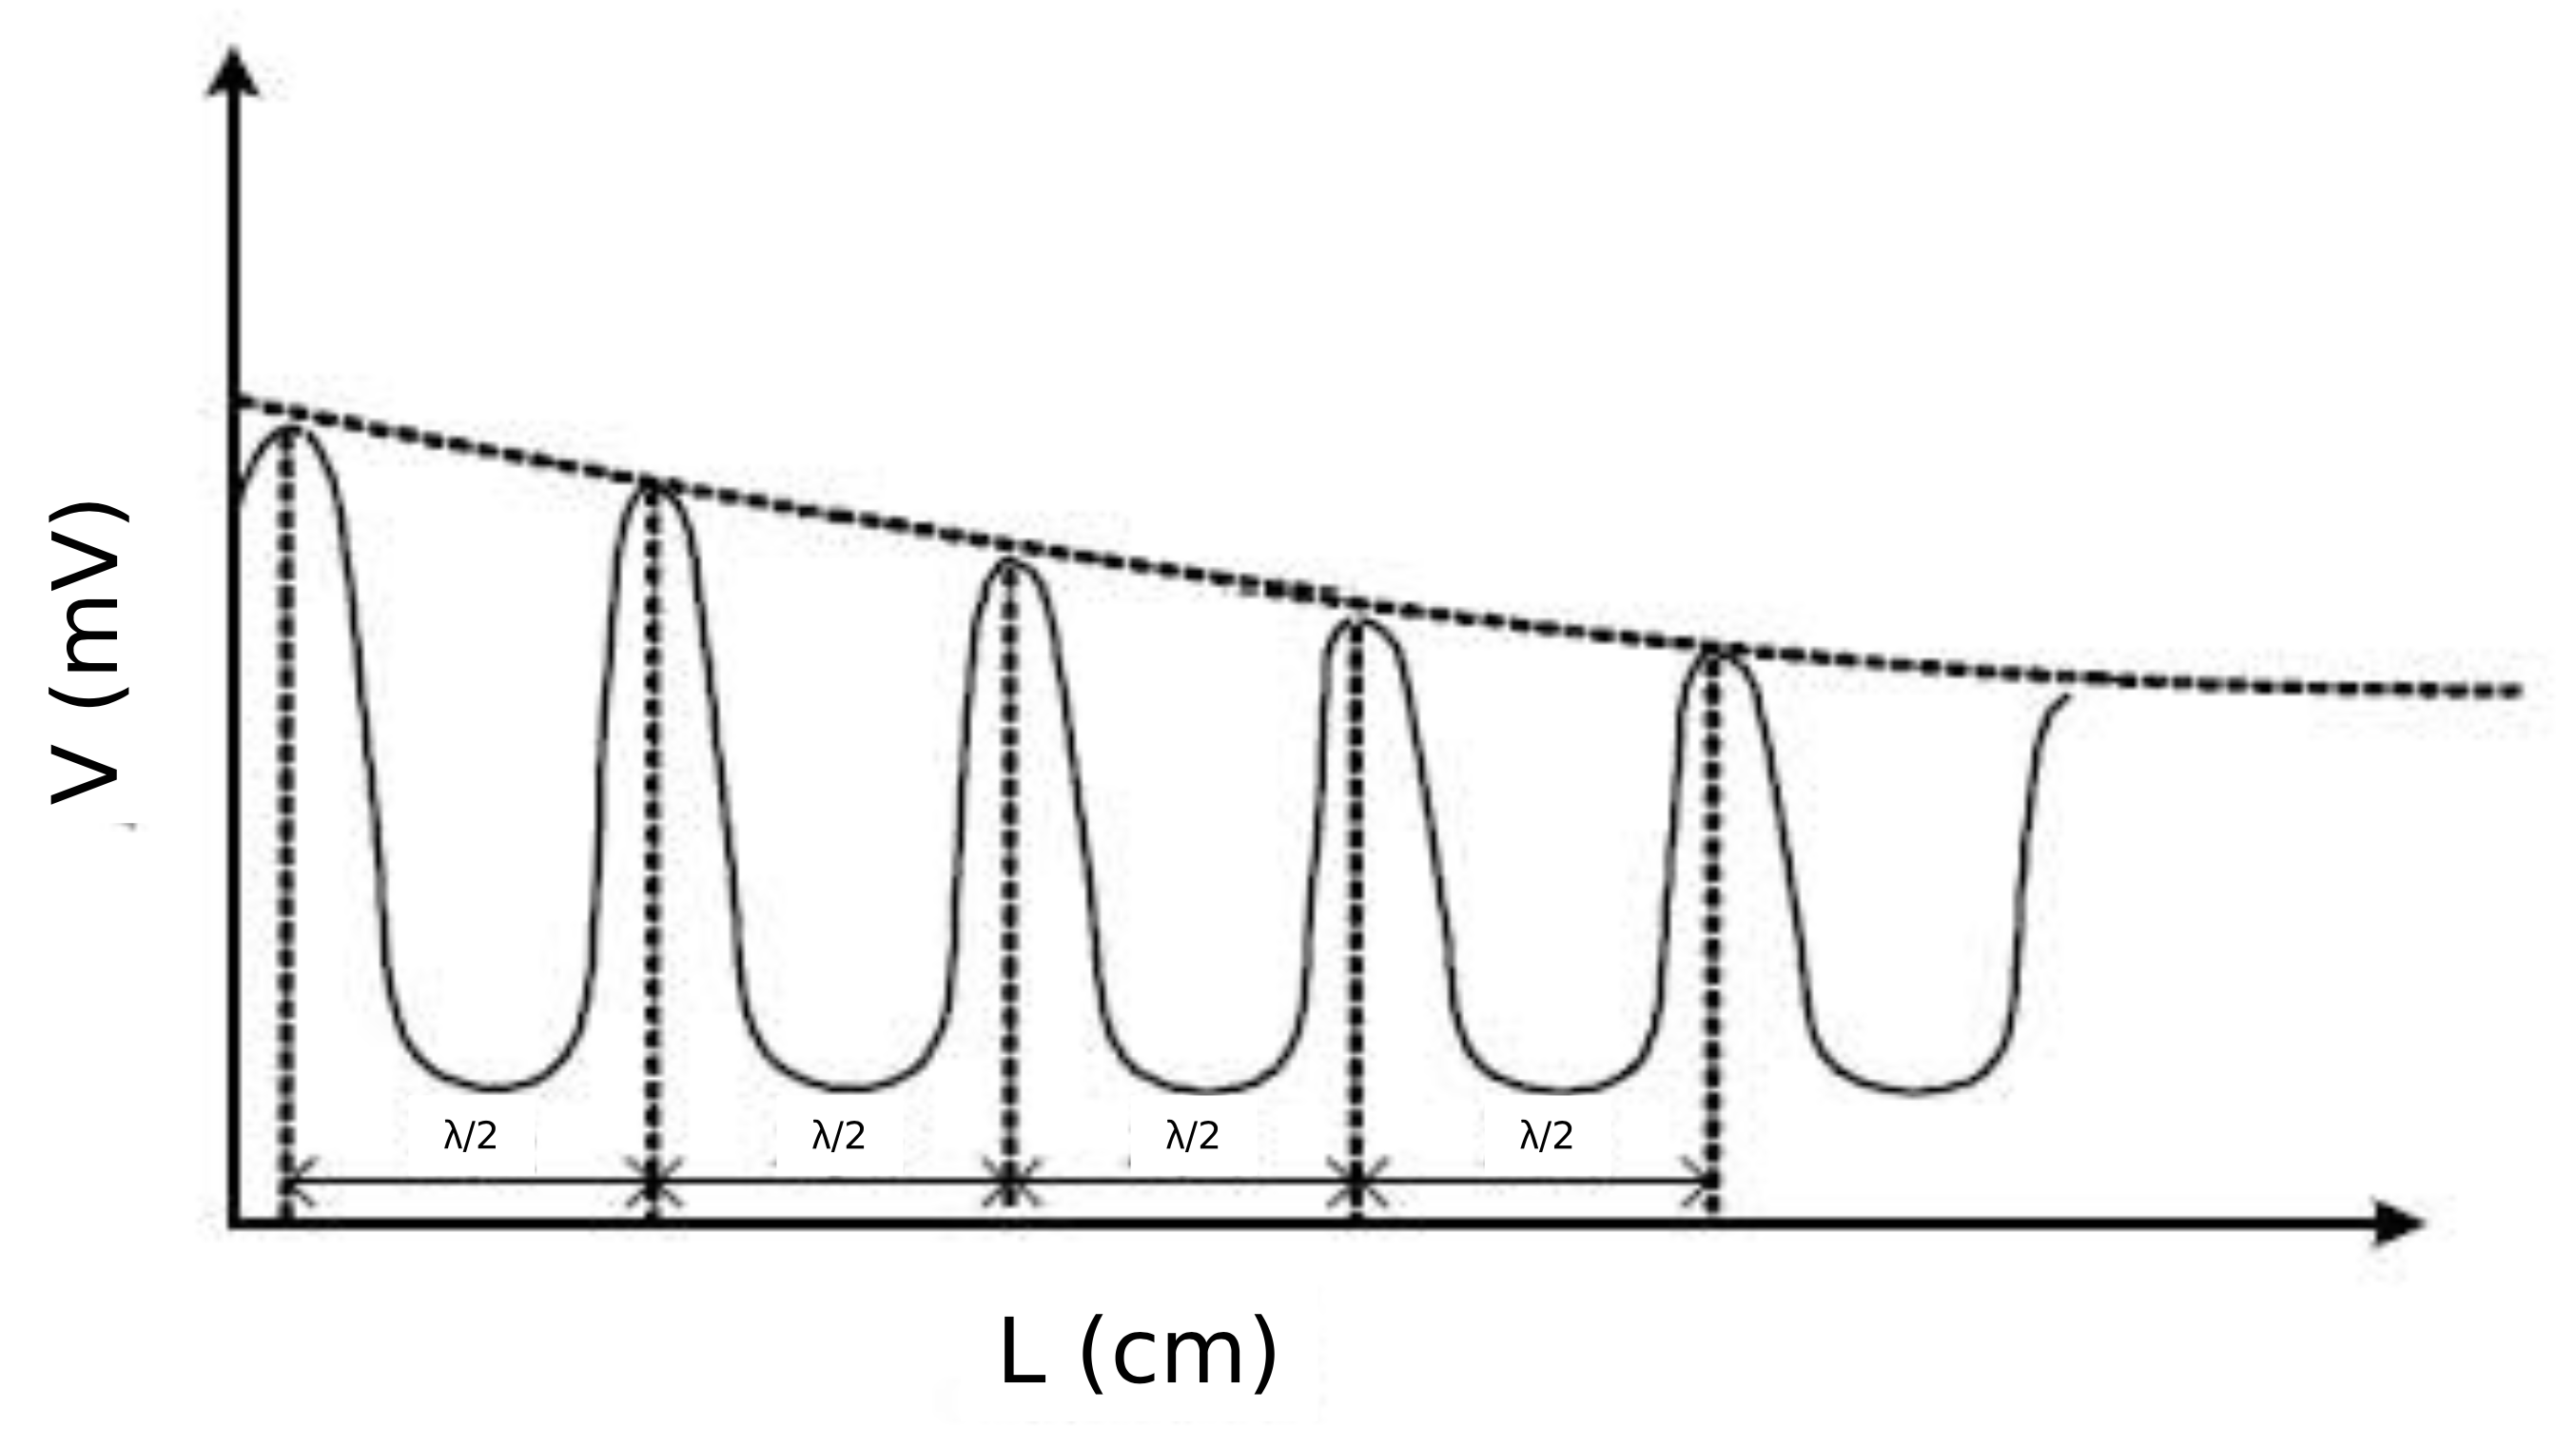
\includegraphics[width=12cm]{fig/r}
    \caption{Relation between the signal voltage and the distance}\label{vL}
\end{figure}

\subsubsection{Phase-comparison method}

If the phase of the wave at two points on the wave propagation direction is
equal, then the distance between these points L has to be a multiple of the
wavelength, \emph{i.e.} 
    
\[
    L=n\lambda,
\]

where $n=1,2,\cdots$. The experimental setup for the phase comparison method
is the same as in the previous method (Figure \ref{app}). Lissajous figures
are used to identify the values of L. Lissajous figures (or Lissajous
curves) are trajectories of a particle that moves in a plane so that
\emph{i.e.} it moves in a harmonic motion independently along two
perpendicular directions (for example the axes x and y of a Cartesian
coordinate system), so that $\textbf{r}(t) = (A_x cos(\omega_x t + \phi_x
),\ A_y cos(\omega_y t + \phi_y ))$. When the two superimposed harmonic
motions have identical frequency $\omega x = \omega y$ and phase difference
$|\phi x - \phi y | = n\pi$, where $n = 0, 1, 2,\cdots$, the Lissajous
figure will show as a straight line. For other values of the phase
difference the figures will have an elliptical shape.\\ 

\subsubsection{Time-difference method}

When an ultrasonic pulse signal emitted by $S_1$ arrives at $S_2$, it is
received and returned back to the processor. By contrasting the original
signal with the received one, one can measure the time needed for the sound
to travel from $S_1$ to $S_2$ over a distance of L. When the values of $L$
and $t$ are known, the phase speed of sound can be found from Eq.
\ref{vlt}.
    
\subsubsection{Successive difference method}

The successive difference method is an effective method to increase the
accuracy of the average value calculated from a series of measurement data.
In this experiment, the usual method of calculating the average value,
illustrated by the formula 

\begin{equation}\label{equ_suc} 
\frac{\bar{\lambda}}{2}
=\frac{[(L_1-L_0)+(L_2-L_1)+\cdots+(L_n-L_{n-1})]}{n}
=\frac{L_n-L_0}{n},
\end{equation} 

will be modified, because as Eq.~\ref{equ_suc} shows, the average value of
the wavelength is determined only by the first and the last value, $L_0$ and
$L_n$. 

A modification of the formula by rearranging terms as
\begin{equation}\label{equ_suc}
    n\frac{\bar{\lambda}}{2}
    =\frac{\Sigma_{i=1}^{n}(L_{n+i}-L_i)}{n},
\end{equation}
produces more accurate results, as each value contributes to the final
result. 